\documentclass[twoside]{book}

\usepackage[paperwidth=148mm, paperheight=210mm]{geometry}
\usepackage{fontspec}
%\usepackage[latin1]{inputenc}
\usepackage[latin.medieval, french]{babel}
\usepackage[strict]{changepage}
\usepackage{fancyhdr}
\usepackage{paracol}
\usepackage{tableof}
\usepackage{setspace}
\usepackage{alltt}
\usepackage{titlesec}
\usepackage{xcolor}
\usepackage{xstring}
\usepackage{enumitem}

%%%%%%%%%%%%%%%%%%%%%%%%%%%%%%%%%%%%%%%%%%%%%%%%%%% Mise ne page %%%%%%%%%%%%%%%%%%%%%%%%%%%%%%
% on numérote les nbp par page et non globalement
\usepackage[perpage]{footmisc}

% définition des en-têtes et pieds de page
\pagestyle{empty}
\fancyhead{}
\fancyfoot{}
\renewcommand{\headrulewidth}{0pt}
\setlength{\headheight}{10pt}
\fancyhead[RO]{\small\thepage}
\fancyhead[LE]{\small\thepage}
% la commande titres permet de changer les titres de gauche et de droite.
\newcommand{\titres}[2]{
	\renewcommand{\rightmark}{\textcolor{red}{\sc #2}}
	\renewcommand{\leftmark}{\textcolor{red}{\sc #1}}
}
\titres{}{}

% pas d'indentation
\setlength{\parindent}{0mm}

\geometry{
inner=25mm,
outer=12mm,
top=15mm,
bottom=15mm,
headsep=3mm,
}

%%%%%%%%%%%%%%%%%%%%%%%%%%%%%%%%%%%%%%%%%%%%%%%%% Options gregorio %%%%%%%%%%%%%%%%%%%%%%%%%

\usepackage[forcecompile]{gregoriotex}
%\usepackage{gregoriotex}

%% style général de gregorio :
% lignes rouges, commenter pour du noir
\gresetlinecolor{gregoriocolor}

% texte <alt> (au-dessus de la portée) en rouge et en petit, avec réglage de sa position verticale
\grechangestyle{abovelinestext}{\color{gregoriocolor}\footnotesize}
\newcommand{\altraise}{-2.4mm}
\grechangedim{abovelinestextraise}{\altraise}{scalable}

% taille des initiales
\newcommand{\initialsize}[1]{
    \grechangestyle{initial}{\fontspec{Zallman}\fontsize{#1}{#1}\selectfont}
}
\newcommand{\defaultinitialsize}{32}
\initialsize{\defaultinitialsize}
% espace avant et après les initiales
\newcommand{\initialspace}[1]{
  \grechangedim{afterinitialshift}{#1}{scalable}
  \grechangedim{beforeinitialshift}{#1}{scalable}
}
\newcommand{\defaultinitialspace}{0cm}
\initialspace{\defaultinitialspace}


% on définit le système qui capture des headers pour générer des annotations
% cette commande sera appelée pour définir des abréviations ou autres substitutions
\newcommand{\resultat}{}
\newcommand{\abbrev}[3]{
  \IfSubStr{#1}{#2}{ \renewcommand{\resultat}{#3} }{}
}
\newcommand{\officepartannotation}[1]{
  \renewcommand{\resultat}{#1}
  \abbrev{#1}{ntro}{ {Intr.} }
  \abbrev{#1}{espo}{Resp.}
  \abbrev{#1}{ll}{All.}
  \abbrev{#1}{act}{Tract.}
  \abbrev{#1}{equen}{Seq.}
  \abbrev{#1}{ffert}{Off.}
  \abbrev{#1}{ommun}{Co.}
  \abbrev{#1}{ntip}{Ant.}
  \abbrev{#1}{ntic}{Cant.}
  \abbrev{#1}{Toni Communes}{}
  \abbrev{#1}{yrial}{}
  \greannotation{\resultat}
}
\newcommand{\modeannotation}[1]{
  \renewcommand{\resultat}{#1}
  \abbrev{#1}{1}{ {\sc i} }
  \abbrev{#1}{2}{ {\sc ii} }
  \abbrev{#1}{3}{ {\sc iii} }
  \abbrev{#1}{4}{ {\sc iv} }
  \abbrev{#1}{5}{ {\sc v} }
  \abbrev{#1}{6}{ {\sc vi} }
  \abbrev{#1}{7}{ {\sc vii} }
  \abbrev{#1}{8}{ {\sc viii} }
  \greannotation{\resultat}
}
\gresetheadercapture{office-part}{officepartannotation}{}
\gresetheadercapture{mode}{modeannotation}{string}

%%%%%%%%%%%%%%%%%%%%%%%%%%%%%%%%%%%%%%%%%%%%%% Graphisme %%%%%%%%%%%%%%%%%%%%%%%%%%%
% on définit l'échelle générale

\newcommand{\echelle}{0.85}

% on centre les titres et on ne les numérote pas
\titleformat{\section}[block]{\Large\filcenter\sc}{}{}{}
\titleformat{\subsection}[block]{\large\filcenter\sc}{}{}{}
\titleformat{\paragraph}[block]{\filcenter\sc}{}{}{}
\setcounter{secnumdepth}{0}
% on diminue l'espace avant les titres
\titlespacing*{\paragraph}{0pt}{1ex}{.6ex}

% commandes versets, repons et croix
\newcommand{\vv}{\textcolor{red}{\fontspec[Scale=\echelle]{Charis SIL}℣.\hspace{3mm}}}
\newcommand{\rr}{\textcolor{red}{\fontspec[Scale=\echelle]{Charis SIL}℟.\hspace{3mm}}}
\newcommand{\cc}{\textcolor{red}{\fontspec[Scale=\echelle]{FreeSerif}\symbol{"2720}~}}
\renewcommand{\aa}{\textcolor{red}{\fontspec[Scale=\echelle]{Charis SIL}\Abar.\hspace{3mm}}}

% commandes diverses
\newcommand{\antiphona}{\textcolor{red}{\noindent Antiphona.\hspace{4mm}}}
\newcommand{\antienne}{\textcolor{red}{\noindent Antienne.\hspace{4mm}}}
\newcommand{\rubrique}[1]{\textcolor{red}{\emph{#1}}}
\newcommand{\saut}{\\ \null \hspace{1cm}}
\newcommand{\minisaut}{\\ \null \hspace{4mm}}
\newcommand{\sautRV}{\\ \null \hspace{5.95mm}}
\newcommand{\petitvspace}{\vspace{2mm}}
\newcommand{\microvspace}{\vspace{0.8mm}}
% pour affichier 1 en rouge et un peu d'espace
\newcommand{\un}{{\color{gregoriocolor} 1~~~}}

% abréviations
\newcommand{\tpalleluia}{\rubrique{(T.P.} \mbox{Allelúia.\rubrique{)}}}
\newcommand{\tpalleluiafr}{\rubrique{(T.P.} \mbox{Alléluia.\rubrique{)}}}

\newcommand{\tqomittitur}{{\small \rubrique{(In Tempore Quadragesimæ ommittitur} Allelúia.\rubrique{)}}}
\newcommand{\careme}{{\small \rubrique{(Pendant le Carême on omet l'}Alléluia.\rubrique{)}}}

% environnement hymne : alltt + normalfont + marges custom
\newenvironment{hymne}
  {
  \begin{adjustwidth}{1.6cm}{1mm}
  \begin{alltt}\normalfont
  }
  {
  \end{alltt}
  \end{adjustwidth}
  }
  
% la commande \u permet de souligner les inflexions
\let\u\underline

% on définit la police par défaut
\setmainfont[Ligatures=TeX, Scale=\echelle]{Charis SIL}
%renderer=ICU a l'air de ne plus marcher...
%\setmainfont[Renderer=ICU, Ligatures=TeX, Scale=\echelle]{Charis SIL}
\setstretch{0.9}

% paramétrage de paracol en mode 2 colonnes par page : taille des colonnes, séparateur
\columnratio{0.5}
\setlength{\columnsep}{1.5em}
\setlength{\columnseprule}{0.3pt}

\begin{document}

% ceci est pour conserver une numérotation ordinaire malgré paracol
\twosided[pb]

\begin{titlepage}
\centering\null

\vspace{1cm}

{\scshape\LARGE In Annuntiatione Beatæ Mariæ Virginis}

\vspace{2cm}
{\scshape\Large Ad Matutinum}

\vspace{5cm}

{\scshape\LARGE L'Annonciation à la Sainte Vierge Marie}

\vspace{2cm}
{\scshape\Large À Matines}


\end{titlepage}

\null\newpage

% tolérance infinie sur les sauts de lignes pour les colonnes étroites
\sloppy

\begin{paracol}{2}
\vv Dómine, lábia \cc mea apéries. \\
\rr Et os meum annuntiábit laudem tuam. \\
\vv Deus \cc in adjutórium meum inténde. \\
\rr Dómine, ad adjuvándum me festína. \\
\vv Glória Patri, et Fílio, et Spirítui Sancto. \\
\rr Sicut erat in princípio, et nunc, et semper, et in sǽcula sæculórum. Amen. Laus tibi, Dómine, Rex ætérnæ glóriæ.
\switchcolumn
\vv Seigneur, Vous ouvrirez mes lèvres. \\
\rr Et ma bouche annoncera Votre louange. \\
\vv Dieu, venez à mon aide. \\
\rr Seigneur, hâtez-vous de me secourir. \\
\vv Gloire au Père, au Fils, et au Saint-Esprit. \\
\rr Comme il était au commencement, maintenant et toujours, et dans les siècles des siècles. Ainsi soit-il. Louange à Vous Seigneur, Roi d'éternelle gloire.
\end{paracol}

\section{Invitatoire}

\gregorioscore{partitions/Invitatorium.gabc}

~

\section{Hymne}
\gregorioscore{partitions/hy--quem_terra_pontus_aethera--ad_matutinum_sub_ritu_monastico.gabc}

\begin{paracol}{2}
\begin{alltt}\normalfont    Celui que terre, mer, astres
    vénèrent, adorent, annoncent,
    Celui qui régit ce triple monde,
    Marie le porte caché dans son sein.

    Celui que lune, soleil et toutes choses
    servent en tout temps,
    est porté par le sein d’une jeune vierge,
    toute pénétrée de la grâce céleste.\end{alltt}
\switchcolumn
\begin{alltt}\normalfont    La bienheureuse mère, par la grâce,
    dans l’arche de son sein,
    renferme l’Artisan suprême
    qui tient le monde dans sa main

    Bienheureuse, à la parole du ciel,
    féconde par le Saint-Esprit,
    et son sein donne au monde
    le désiré des nations.\end{alltt}
\end{paracol}
\begin{alltt}\normalfont                                     Ô Jésus, gloire à vous
                                     qui êtes né de la Vierge,
                                     ainsi qu’au Père et à l’Esprit nourricier,
                                     dans les siècles éternels.
                                     Ainsi soit-il.\end{alltt}

\section{Premier nocturne}

\subsection{Psaume 8}

\gregorioscore{partitions/an1--benedicta_tu_in_mulieribus--nocturnale_2002.gabc}
\gresetinitiallines{0}
\gregorioscore{partitions/ps1.gabc}
\gresetinitiallines{1}
\aa \emph{Vous êtes bénie entre les femmes et le fruit de votre sein est béni.}

\un \emph{Ô Seigneur, notre Dieu, qu'il est grand ton nom par toute la terre !}
\begin{paracol}{2}
\begin{enumerate}[wide, itemsep=0mm, labelwidth=!, labelindent=0pt, label=\color{gregoriocolor}\theenumi]
\setcounter{enumi}{1}
\selectlanguage{latin}
\item Quóniam eleváta est magnificén\textit{ti}\textit{a} \textbf{tu}a,~* \textit{su}\textit{per} \textbf{cæ}los.
\item Ex ore infántium et lacténtium perfecísti laudem propter ini\textit{mí}\textit{cos} \textbf{tu}os,~* ut déstruas inimí\textit{cum} \textit{et} \textit{ul}\textbf{tó}rem.
\item Quóniam vidébo cælos tuos, ópera digitó\textit{rum} \textit{tu}\textbf{ó}rum:~* lunam et stellas, \textit{quæ} \textit{tu} \textit{fun}\textbf{dás}ti.
\item Quid est homo quod me\textit{mor} \textit{es} \textbf{e}jus?~* aut fílius hóminis, quóniam \textit{ví}\textit{si}\textit{tas} \textbf{e}um?
\item Minuísti eum paulo minus ab Angelis,~† glória et honóre coro\textit{nás}\textit{ti} \textbf{e}um:~* et constituísti eum super ópera má\textit{nu}\textit{um} \textit{tu}\textbf{á}rum.
\item Omnia subjecísti sub pé\textit{di}\textit{bus} \textbf{e}jus,~* oves et boves univérsas: ínsuper et \textit{pé}\textit{co}\textit{ra} \textbf{cam}pi.
\item Vólucres cæli, et \textit{pi}\textit{sces} \textbf{ma}ris,~* qui perámbulant \textit{sé}\textit{mi}\textit{tas} \textbf{ma}ris.
\item Dómine, Dó\textit{mi}\textit{nus} \textbf{nos}ter,~* quam admirábile est nomen tuum in u\textit{ni}\textit{vér}\textit{sa} \textbf{ter}ra!
\item Glória Pa\textit{tri}, \textit{et} \textbf{Fí}lio,~* et Spi\textit{rí}\textit{tu}\textit{i} \textbf{Sanc}to.
\item Sicut erat in princípio, et \textit{nunc}, \textit{et} \textbf{sem}per,~* et in sǽcula sæ\textit{cu}\textit{ló}\textit{rum}. \textbf{A}men.
\selectlanguage{french}
\end{enumerate}
\switchcolumn
\begin{enumerate}[wide, itemsep=0mm, labelwidth=!, labelindent=0pt, before=\itshape, label=\color{gregoriocolor}\theenumi]
\setcounter{enumi}{1}
\item Jusqu'aux cieux, ta splendeur est chantée.
\item par la bouche des enfants, des tout-petits : rempart que tu opposes à l'adversaire, où l'ennemi se brise en sa révolte.
\item À voir ton ciel, ouvrage de tes doigts, la lune et les étoiles que tu fixas,
\item qu'est-ce que l'homme pour que tu penses à lui, le fils d'un homme, que tu en prennes souci ?
\item Tu l'as voulu un peu moindre qu'un dieu, le couronnant de gloire et d'honneur ;
\item tu l'établis sur les oeuvres de tes mains, tu mets toute chose à ses pieds :
\item les troupeaux de boeufs et de brebis, et même les bêtes sauvages,
\item les oiseaux du ciel et les poissons de la mer, tout ce qui va son chemin dans les eaux.
\item O Seigneur, notre Dieu, qu'il est grand ton nom par toute la terre !
\item Gloire au Père, au Fils, et au Saint-Esprit.
\item Comme elle était au commencement, maintenant et toujours, dans les siècles des siècles. Ainsi-soit il.
\end{enumerate}
\end{paracol}

\subsection{Psaume 18}

\gregorioscore{partitions/an2--sicut_myrrha--nocturnale_2002.gabc}
\gresetinitiallines{0}
\gregorioscore{partitions/ps2.gabc}
\gresetinitiallines{1}
\aa \emph{Comme une myrrhe de choix vous avez exhalé un parfum suave, ô sainte Mère de Dieu.}

\un \emph{Les cieux proclament la gloire de Dieu, le firmament raconte l'ouvrage de ses mains.}
\begin{paracol}{2}
\begin{enumerate}[wide, itemsep=0mm, labelwidth=!, labelindent=0pt, label=\color{gregoriocolor}\theenumi]
\setcounter{enumi}{1}
\selectlanguage{latin}
\item Dies diéi e\textit{rúc}\textit{tat} \textbf{ver}bum,~* et nox nocti ín\textit{di}\textit{cat} \textit{sci}\textbf{én}tiam.
\item Non sunt loquélæ, ne\textit{que} \textit{ser}\textbf{mó}nes,~* quorum non audiántur \textit{vo}\textit{ces} \textit{e}\textbf{ó}rum.
\item In omnem terram exívit so\textit{nus} \textit{e}\textbf{ó}rum:~* et in fines orbis terræ \textit{ver}\textit{ba} \textit{e}\textbf{ó}rum.
\item In sole pósuit taberná\textit{cu}\textit{lum} \textbf{su}um:~* et ipse tamquam sponsus procédens de \textit{thá}\textit{la}\textit{mo} \textbf{su}o.
\item Exsultávit ut gigas ad cur\textit{rén}\textit{dam} \textbf{vi}am,~* a summo cælo e\textit{grés}\textit{si}\textit{o} \textbf{e}jus.
\item Et occúrsus ejus usque ad \textit{sum}\textit{mum} \textbf{e}jus:~* nec est qui se abscóndat a \textit{ca}\textit{ló}\textit{re} \textbf{e}jus.
\item Lex Dómini immaculáta, con\textit{vér}\textit{tens} \textbf{á}nimas:~* testimónium Dómini fidéle, sapiénti\textit{am} \textit{præ}\textit{stans} \textbf{pár}vulis.
\item Justítiæ Dómini rectæ, lætifi\textit{cán}\textit{tes} \textbf{cor}da:~* præcéptum Dómini lúcidum il\textit{lú}\textit{mi}\textit{nans} \textbf{ó}culos.
\item Timor Dómini sanctus, pérmanens in sǽ\textit{cu}\textit{lum} \textbf{sǽ}culi:~* judícia Dómini vera, justificáta \textit{in} \textit{se}\textit{met}\textbf{íp}sa.
\item Desiderabília super aurum et lápidem preti\textit{ó}\textit{sum} \textbf{mul}tum:~* et dulcióra su\textit{per} \textit{mel} \textit{et} \textbf{fa}vum.
\item Etenim servus tuus cus\textit{tó}\textit{dit} \textbf{e}a,~* in custodiéndis illis retri\textit{bú}\textit{ti}\textit{o} \textbf{mul}ta.
\item Delícta quis intélligit?~† ab occúltis \textit{me}\textit{is} \textbf{mun}da me:~* et ab aliénis par\textit{ce} \textit{ser}\textit{vo} \textbf{tu}o.
\item Si mei non fúerint domináti, tunc immacu\textit{lá}\textit{tus} \textbf{e}ro:~* et emundábor a \textit{de}\textit{líc}\textit{to} \textbf{má}ximo.
\item Et erunt ut compláceant elóquia \textit{o}\textit{ris} \textbf{me}i:~* et meditátio cordis mei in conspéc\textit{tu} \textit{tu}\textit{o} \textbf{sem}per.
\item Dómine, ad\textit{jú}\textit{tor} \textbf{me}us,~* et \textit{red}\textit{émp}\textit{tor} \textbf{me}us.
\item Glória Pa\textit{tri}, \textit{et} \textbf{Fí}lio,~* et Spi\textit{rí}\textit{tu}\textit{i} \textbf{Sanc}to.
\item Sicut erat in princípio, et \textit{nunc}, \textit{et} \textbf{sem}per,~* et in sǽcula sæ\textit{cu}\textit{ló}\textit{rum}. \textbf{A}men.
\selectlanguage{french}
\end{enumerate}
\switchcolumn
\begin{enumerate}[wide, itemsep=0mm, labelwidth=!, labelindent=0pt, before=\itshape, label=\color{gregoriocolor}\theenumi]
\setcounter{enumi}{1}
\item Le jour au jour en livre le récit et la nuit à la nuit en donne connaissance.
\item Pas de paroles dans ce récit, pas de voix qui s'entende;
\item mais sur toute la terre en paraît le message et la nouvelle, aux limites du monde. 
\item Là, se trouve la demeure du soleil : tel un époux, il paraît hors de sa tente,
\item il s'élance en conquérant joyeux. Il paraît où commence le ciel,
\item il s'en va jusqu'où le ciel s'achève : rien n'échappe à son ardeur.
\item La loi du Seigneur est parfaite, qui redonne vie ; la charte du Seigneur est sûre, qui rend sages les simples.
\item Les préceptes du Seigneur sont droits, ils réjouissent le cœur ; le commandement du Seigneur est limpide, il clarifie le regard.
\item La crainte qu'il inspire est pure, elle est là pour toujours ; les décisions du Seigneur sont justes et vraiment équitables :
\item plus désirables que l'or, qu'une masse d'or fin, plus savoureuses que le miel qui coule des rayons.
\item Aussi ton serviteur en est illuminé ; à les garder, il trouve son profit.
\item Qui peut discerner ses erreurs ? Purifie-moi de celles qui m'échappent.
\item Préserve aussi ton serviteur de l'orgueil : qu'il n'ait sur moi aucune emprise. Alors je serai sans reproche, pur d'un grand péché.
\item Accueille les paroles de ma bouche, le murmure de mon cœur ; qu'ils parviennent devant toi, 
\item Seigneur, mon rocher, mon défenseur !
\item Gloire au Père, au Fils, et au Saint-Esprit.
\item Comme elle était au commencement, maintenant et toujours, dans les siècles des siècles. Ainsi-soit il.
\end{enumerate}
\end{paracol}

\subsection{Psaume 23}

\gregorioscore{partitions/an3--ante_torum--nocturnale_2002.gabc}
\gresetinitiallines{0}
\gregorioscore{partitions/ps3.gabc}
\gresetinitiallines{1}
\aa \emph{Devant le trône de cette Vierge, chantez-nous souvent de doux cantiques qui nous rappellent ses saintes actions.}

\un \emph{Au Seigneur, le monde et sa richesse, la terre et tous ses habitants !}
\begin{paracol}{2}
\begin{enumerate}[wide, itemsep=0mm, labelwidth=!, labelindent=0pt, label=\color{gregoriocolor}\theenumi]
\setcounter{enumi}{1}
\selectlanguage{latin}
\item Quia ipse super mária fun\textit{dá}\textit{vit} \textbf{e}um:~* et super flúmina præ\textit{pa}\textit{rá}\textit{vit} \textbf{e}um.
\item Quis ascéndet in \textit{mon}\textit{tem} \textbf{Dó}mini?~* aut quis stabit in lo\textit{co} \textit{sanc}\textit{to} \textbf{e}jus?
\item Innocens mánibus et mundo corde,~† qui non accépit in vano á\textit{ni}\textit{mam} \textbf{su}am,~* nec jurávit in dolo \textit{pró}\textit{xi}\textit{mo} \textbf{su}o.
\item Hic accípiet benedictió\textit{nem} \textit{a} \textbf{Dó}mino:~* et misericórdiam a Deo, sa\textit{lu}\textit{tá}\textit{ri} \textbf{su}o.
\item Hæc est generátio quærén\textit{ti}\textit{um} \textbf{e}um,~* quæréntium fáci\textit{em} \textit{De}\textit{i} \textbf{Ja}cob.
\item Attóllite portas, príncipes, vestras,~† et elevámini, portæ \textit{æ}\textit{ter}\textbf{ná}les:~* et intro\textit{í}\textit{bit} \textit{Rex} \textbf{gló}riæ.
\item Quis est iste Rex glóriæ?~† Dóminus for\textit{tis} \textit{et} \textbf{pot}ens:~* Dóminus \textit{pot}\textit{ens} \textit{in} \textbf{prǽ}lio.
\item Attóllite portas, príncipes, vestras,~† et elevámini, portæ \textit{æ}\textit{ter}\textbf{ná}les:~* et intro\textit{í}\textit{bit} \textit{Rex} \textbf{gló}riæ.
\item Quis est is\textit{te} \textit{Rex} \textbf{gló}riæ?~* Dóminus virtútum ip\textit{se} \textit{est} \textit{Rex} \textbf{gló}riæ.
\item Glória Pa\textit{tri}, \textit{et} \textbf{Fí}lio,~* et Spi\textit{rí}\textit{tu}\textit{i} \textbf{Sanc}to.
\item Sicut erat in princípio, et \textit{nunc}, \textit{et} \textbf{sem}per,~* et in sǽcula sæ\textit{cu}\textit{ló}\textit{rum}. \textbf{A}men.
\selectlanguage{french}
\end{enumerate}
\switchcolumn
\begin{enumerate}[wide, itemsep=0mm, labelwidth=!, labelindent=0pt, before=\itshape, label=\color{gregoriocolor}\theenumi]
\setcounter{enumi}{1}
\item C'est lui qui l'a fondée sur les mers et la garde inébranlable sur les flots.
\item Qui peut gravir la montagne du Seigneur et se tenir dans le lieu saint ?
\item L'homme au cœur pur, aux mains innocentes, qui ne livre pas son âme aux idoles, et ne dit pas de faux serments.
\item Il obtient, du Seigneur, la bénédiction, et de Dieu son Sauveur, la justice.
\item Voici le peuple de ceux qui le cherchent ! Voici Jacob qui recherche ta face !
\item Portes, levez vos frontons, élevez-vous, portes éternelles : qu'il entre, le roi de gloire !
\item Qui est ce roi de gloire ? C'est le Seigneur, le fort, le vaillant, le Seigneur, le vaillant des combats.
\item Portes, levez vos frontons, levez-les, portes éternelles : qu'il entre, le roi de gloire !
\item Qui donc est ce roi de gloire ? C'est le Seigneur, Dieu de l'univers ; c'est lui, le roi de gloire.
\item Gloire au Père, au Fils, et au Saint-Esprit.
\item Comme elle était au commencement, maintenant et toujours, dans les siècles des siècles. Ainsi-soit il.
\end{enumerate}
\end{paracol}

\subsection{Versicule}
\begin{paracol}{2}
\vv Spécie tua et pulchritúdine tua. \\
\rr Inténde, próspere procéde, et regna. \\
\vv Pater noster... \rubrique{(secrètement)} Et ne nos indúcas in tentatiónem. \\
\rr Sed líbera nos a malo. \\
\vv Exáudi, Dómine Iesu Christe, preces servórum tuórum, et miserére nobis: Qui cum Patre et Spíritu Sancto vivis et regnas in sǽcula sæculórum. \\
\rr Amen.
\switchcolumn
\vv Dans votre gloire et votre beauté. \\
\rr Avancez heureusement, avancez et régnez. \\
\vv Notre Père... Et ne nous laissez pas succomber à la tentation. \\
\rr Mais délivrez-nous du mal. \\
\vv Exaucez, Seigneur Jésus-Christ, les prières de vos serviteurs, et ayez pitié de nous, vous qui vivez et régnez avec le Père et le Saint-Esprit, dans les siècles des siècles. \rr Ainsi soit-il.
\end{paracol}

\subsection{Première leçon}

\begin{paracol}{2}
\vv Jube, domne, benedícere. \\
\vv Benedictióne perpétua benedícat nos Pater ætérnus.\\
\rr Amen.
\switchcolumn
\vv Veuillez, Seigneur, bénir. \\
\vv Que le Père éternel nous bénisse d'une bénédiction perpétuelle. \\
\rr Ainsi soit-il.
\end{paracol}

\paragraph{Lecture du livre d'Isaïe} \rubrique{Is 7 : 10-15}

Le Seigneur parla encore ainsi au roi Acaz :

« Demande pour toi un signe de la part du Seigneur ton Dieu, au fond du séjour des morts ou sur les sommets, là-haut. »

Acaz répondit : « Non, je n’en demanderai pas, je ne mettrai pas le Seigneur à l’épreuve. »

Isaïe dit alors : « Écoutez, maison de David ! Il ne vous suffit donc pas de fatiguer les hommes : il faut encore que vous fatiguiez mon Dieu !

C’est pourquoi le Seigneur lui-même vous donnera un signe : Voici que la vierge est enceinte, elle enfantera un fils, qu’elle appellera Emmanuel (c’est-à-dire : Dieu-avec-nous).

De crème et de miel il se nourrira, jusqu’à ce qu’il sache rejeter le mal et choisir le bien.

\begin{paracol}{2}
\vv Tu autem, Dómine, miserére nobis. \\
\rr Deo grátias.
\switchcolumn
\vv Et vous Seigneur, ayez pitié de nous. \\
\rr Rendons grâces à Dieu.
\end{paracol}

\gregorioscore{partitions/re1--missus_est_gabriel_(resp)--gregofacsimil.gabc}

\emph{\rr L’Ange Gabriel fut envoyé à Marie, vierge qu’avait épousée Joseph, lui portant un message, et la Vierge fut effrayée de la lumière. Ne craignez point, Marie ; vous avez trouvé grâce devant le Seigneur :
Voilà que vous concevrez et que vous enfanterez, et il sera appelé le Fils du Très-Haut.
\\
\vv Je vous salue, Marie, pleine de grâce, le Seigneur est avec vous.}

\subsection{Deuxième leçon}

\begin{paracol}{2}
\vv Jube, domne, benedícere. \\
\vv Unigénitus Dei Fílius nos benedícere et adjuváre dignétur.\\
\rr Amen.
\switchcolumn
\vv Veuillez, Seigneur, bénir. \\
\vv Que le Fils unique de Dieu daigne nous bénir et nous secourir.\\
\rr Ainsi soit-il.
\end{paracol}

\rubrique{Is 11 : 1-5}

Un rameau sortira de la souche de Jessé, père de David, un rejeton jaillira de ses racines.

Sur lui reposera l’esprit du Seigneur : esprit de sagesse et de discernement, esprit de conseil et de force, esprit de connaissance et de crainte du Seigneur – qui lui inspirera la crainte du Seigneur. Il ne jugera pas sur l’apparence ; il ne se prononcera pas sur des rumeurs.

Il jugera les petits avec justice ; avec droiture, il se prononcera en faveur des humbles du pays. Du bâton de sa parole, il frappera le pays ; du souffle de ses lèvres, il fera mourir le méchant.

La justice est la ceinture de ses hanches ; la fidélité est la ceinture de ses reins.

\begin{paracol}{2}
\vv Tu autem, Dómine, miserére nobis. \\
\rr Deo grátias.
\switchcolumn
\vv Et vous Seigneur, ayez pitié de nous. \\
\rr Rendons grâces à Dieu.
\end{paracol}

\newpage
\gregorioscore{partitions/re2--ave_maria_(resp.)--gregofacsimil.gabc}

\emph{\rr Je vous salue, Marie, pleine de grâce ; le Seigneur est avec vous :
l’Esprit-Saint surviendra en vous, et la vertu du Très-Haut vous couvrira de son ombre ; c’est pourquoi la chose sainte qui naîtra de vous sera appelée le Fils de Dieu. \\
\vv Portes, élevez vos frotons, levez-vous, portes éternelles : qu'il entre, le Fils de Dieu.}

\newpage
\subsection{Troisième leçon}

~

\begin{paracol}{2}
\vv Jube, domne, benedícere. \\
\vv Spíritus Sancti grátia illúminet sensus et corda nostra.\\
\rr Amen.
\switchcolumn
\vv Veuillez, Seigneur, bénir. \\
\vv Que la grâce du Saint-Esprit illumine nos esprits et nos cœurs.\\
\rr Ainsi soit-il.
\end{paracol}

\rubrique{Is 35 : 1-7}

Le désert et la terre de la soif, qu’ils se réjouissent ! Le pays aride, qu’il exulte et fleurisse comme la rose,
qu’il se couvre de fleurs des champs, qu’il exulte et crie de joie ! La gloire du Liban lui est donnée, la splendeur du Carmel et du Sarone. On verra la gloire du Seigneur, la splendeur de notre Dieu.

Fortifiez les mains défaillantes, affermissez les genoux qui fléchissent,
dites aux gens qui s’affolent : « Soyez forts, ne craignez pas. Voici votre Dieu : c’est la vengeance qui vient, la revanche de Dieu. Il vient lui-même et va vous sauver. »

Alors se dessilleront les yeux des aveugles, et s’ouvriront les oreilles des sourds.

Alors le boiteux bondira comme un cerf, et la bouche du muet criera de joie ; car l’eau jaillira dans le désert, des torrents dans le pays aride.

La terre brûlante se changera en lac, la région de la soif, en eaux jaillissantes.

\begin{paracol}{2}
\vv Tu autem, Dómine, miserére nobis. \\
\rr Deo grátias.
\switchcolumn
\vv Et vous Seigneur, ayez pitié de nous. \\
\rr Rendons grâces à Dieu.
\end{paracol}

\gregorioscore{partitions/re3--suscipe_verbum_(resp.)--gregofacsimil.gabc}

\emph{\rr Recevez, Vierge Marie, la parole du Seigneur, qui vous est transmise par un Ange : vous concevrez et enfanterez Dieu et homme tout ensemble, Et ainsi vous serez appelée bénie entre toutes les femmes. \\
\vv Je vous salue Marie, pleine de grâce, le Seigneur est avec vous.}

\section{Deuxième nocturne}

\subsection{Psaume 44}

\gregorioscore{partitions/an4--specie_tua_(ant)--nocturnale_2002.gabc}
\gresetinitiallines{0}
\gregorioscore{partitions/ps4.gabc}
\gresetinitiallines{1}
\aa \emph{Dans votre dignité et votre beauté, avancez, avancez avec succès et régnez.}

\un \emph{D'heureuses paroles jaillissent de mon cœur quand je dis mes poèmes pour le roi.}
\begin{paracol}{2}

\begin{enumerate}[wide, itemsep=0mm, labelwidth=!, labelindent=0pt, label=\color{gregoriocolor}\theenumi]
\setcounter{enumi}{1}
\selectlanguage{latin}
\item Lingua mea \textbf{cá}lamus \textbf{scri}bæ:~* velóci\textbf{ter} scri\textbf{bén}tis.
\item Speciósus forma præ fíliis hóminum,~† diffúsa est grátia in \textbf{lá}biis \textbf{tu}is:~* proptérea benedíxit te Deus \textbf{in} æ\textbf{tér}num.
\item Accíngere gládio tuo super \textbf{fe}mur \textbf{tu}um,~* \textbf{pot}en\textbf{tís}sime.
\item Spécie tua et pulchri\textbf{tú}dine \textbf{tu}a:~* inténde, próspere pro\textbf{cé}de, et \textbf{re}gna.
\item Propter veritátem, et mansuetúdinem, \textbf{et} jus\textbf{tí}tiam:~* et dedúcet te mirabíliter \textbf{déx}tera \textbf{tu}a.
\item Sagíttæ tuæ acútæ, pópuli \textbf{sub} te \textbf{ca}dent:~* in corda inimi\textbf{có}rum \textbf{Re}gis.
\item Sedes tua, Deus, in \textbf{sǽ}culum \textbf{sǽ}culi:~* virga directiónis virga \textbf{re}gni \textbf{tu}i.
\item Dilexísti justítiam, et odísti in\textbf{i}qui\textbf{tá}tem:~* proptérea unxit te, Deus, Deus tuus, óleo lætítiæ præ con\textbf{sór}tibus \textbf{tu}is.
\item Myrrha, et gutta, et cásia a vestiméntis tuis, a dómi\textbf{bus} e\textbf{búr}neis:~* ex quibus delectavérunt te fíliæ regum in ho\textbf{nó}re \textbf{tu}o.
\item Astitit regína a dextris tuis in vestítu \textbf{de}au\textbf{rá}to:~* circúmdata va\textbf{ri}e\textbf{tá}te.
\item Audi, fília, et vide, et inclína \textbf{au}rem \textbf{tu}am:~* et oblivíscere pópulum tuum, et domum \textbf{pa}tris \textbf{tu}i.
\item Et concupíscet Rex de\textbf{có}rem \textbf{tu}um:~* quóniam ipse est Dóminus Deus tuus, et ado\textbf{rá}bunt \textbf{e}um.
\item Et fíliæ Tyri \textbf{in} mu\textbf{né}ribus~* vultum tuum deprecabúntur: omnes \textbf{dí}vites \textbf{ple}bis.
\item Omnis glória ejus fíliæ \textbf{Re}gis ab \textbf{in}tus,~* in fímbriis áureis circumamícta va\textbf{ri}e\textbf{tá}tibus.
\item Adducéntur Regi vírgi\textbf{nes} post \textbf{e}am:~* próximæ ejus affe\textbf{rén}tur \textbf{ti}bi.
\item Afferéntur in lætítia et exsul\textbf{ta}ti\textbf{ó}ne:~* adducéntur in \textbf{tem}plum \textbf{Re}gis.
\item Pro pátribus tuis nati sunt \textbf{ti}bi \textbf{fí}lii:~* constítues eos príncipes super \textbf{om}nem \textbf{ter}ram.
\item Mémores erunt \textbf{nó}minis \textbf{tu}i:~* in omni generatióne et gene\textbf{ra}ti\textbf{ó}nem.
\item Proptérea pópuli confitebúntur tibi \textbf{in} æ\textbf{tér}num:~* et in \textbf{sǽ}culum \textbf{sǽ}culi.
\item Glória \textbf{Pa}tri, et \textbf{Fí}lio,~* et Spi\textbf{rí}tui \textbf{Sanc}to.
\item Sicut erat in princípio, et \textbf{nunc}, et \textbf{sem}per,~* et in sǽcula sæcu\textbf{ló}rum. \textbf{A}men.
\selectlanguage{french}
\end{enumerate}

\switchcolumn
\begin{enumerate}[wide, itemsep=0mm, labelwidth=!, labelindent=0pt, before=\itshape, label=\color{gregoriocolor}\theenumi]
\setcounter{enumi}{1}
\item D'une langue aussi vive que la plume du scribe !
\item Tu es beau, comme aucun des enfants de l'homme, la grâce est répandue sur tes lèvres : oui, Dieu te bénit pour toujours.
\item Guerrier valeureux, porte l'épée de noblesse et d'honneur !
\item Ton honneur, c'est de courir au combat pour la justice, la clémence et la vérité.
\item Ta main jettera la stupeur, les flèches qui déchirent ; 
\item sous tes coups, les peuples s'abattront, les ennemis du roi, frappés en plein cœur.
\item Ton trône est divin, un trône éternel ; ton sceptre royal est sceptre de droiture :
\item tu aimes la justice, tu réprouves le mal. Oui, Dieu, ton Dieu t'a consacré d'une onction de joie, comme aucun de tes semblables ;
\item la myrrhe et l'aloès parfument ton vêtement. Des palais d'ivoire, la musique t'enchante.
\item Parmi tes bien-aimées sont des filles de roi ; à ta droite, la préférée, sous les ors d'Ophir.
\item Écoute, ma fille, regarde et tends l'oreille ; oublie ton peuple et la maison de ton père :
\item le roi sera séduit par ta beauté. Il est ton Seigneur : prosterne-toi devant lui.
\item Alors, fille de Tyr, les plus riches du peuple, chargés de présents, quêteront ton sourire.
\item Fille de roi, elle est là, dans sa gloire, vêtue d'étoffes d'or ;
\item on la conduit, toute parée, vers le roi. Des jeunes filles, ses compagnes, lui font cortège ;
\item on les conduit parmi les chants de fête : elles entrent au palais du roi.
\item À la place de tes pères se lèveront tes fils ; sur toute la terre tu feras d'eux des princes.
\item Je ferai vivre ton nom pour les âges des âges : 
\item que les peuples te rendent grâce, toujours, à jamais !
\item Gloire au Père, au Fils, et au Saint-Esprit.
\item Comme elle était au commencement, maintenant et toujours, dans les siècles des siècles. Ainsi-soit il.
\end{enumerate}

\end{paracol}

\subsection{Psaume 45}

\gregorioscore{partitions/an5--adjuvabit_eam--nocturnale_2002.gabc}
\gresetinitiallines{0}
\gregorioscore{partitions/ps5.gabc}
\gresetinitiallines{1}
\aa \emph{Dieu la protège de son regard : Dieu est au milieu d’elle, elle ne sera pas ébranlée.}

\un \emph{Dieu est pour nous refuge et force, secours dans la détresse, toujours offert.}
\begin{paracol}{2}

\begin{enumerate}[wide, itemsep=0mm, labelwidth=!, labelindent=0pt, label=\color{gregoriocolor}\theenumi]
\setcounter{enumi}{1}
\selectlanguage{latin}
\item Proptérea non timébimus dum tur\textbf{bá}bitur \textbf{ter}ra:~* et transferéntur montes \textbf{in} cor \textbf{ma}ris.
\item Sonuérunt, et turbátæ sunt \textbf{a}quæ e\textbf{ó}rum:~* conturbáti sunt montes in forti\textbf{tú}dine \textbf{e}jus.
\item Flúminis ímpetus lætíficat civi\textbf{tá}tem \textbf{De}i:~* sanctificávit tabernáculum \textbf{su}um Al\textbf{tís}simus.
\item Deus in médio ejus, non \textbf{com}mo\textbf{vé}bitur:~* adjuvábit eam Deus \textbf{ma}ne di\textbf{lú}culo.
\item Conturbátæ sunt Gentes, et incli\textbf{ná}ta sunt \textbf{re}gna:~* dedit vocem suam, \textbf{mo}ta est \textbf{ter}ra.
\item Dóminus vir\textbf{tú}tum no\textbf{bís}cum:~* suscéptor noster \textbf{De}us \textbf{Ja}cob.
\item Veníte, et vidéte ópera Dómini,~† quæ pósuit prodígia \textbf{su}per \textbf{ter}ram:~* áuferens bella usque ad \textbf{fi}nem \textbf{ter}ræ.
\item Arcum cónteret, et con\textbf{frín}get \textbf{ar}ma:~* et scuta com\textbf{bú}ret \textbf{i}gni.
\item Vacáte, et vidéte quóniam \textbf{e}go sum \textbf{De}us:~* exaltábor in Géntibus, et exal\textbf{tá}bor in \textbf{ter}ra.
\item Dóminus vir\textbf{tú}tum no\textbf{bís}cum:~* suscéptor noster \textbf{De}us \textbf{Ja}cob.
\item Glória \textbf{Pa}tri, et \textbf{Fí}lio,~* et Spi\textbf{rí}tui \textbf{Sanc}to.
\item Sicut erat in princípio, et \textbf{nunc}, et \textbf{sem}per,~* et in sǽcula sæcu\textbf{ló}rum. \textbf{A}men.
\selectlanguage{french}
\end{enumerate}

\switchcolumn
\begin{enumerate}[wide, itemsep=0mm, labelwidth=!, labelindent=0pt, before=\itshape, label=\color{gregoriocolor}\theenumi]
\setcounter{enumi}{1}
\item Nous serons sans crainte si la terre est secouée, si les montagnes s'effondrent au creux de la mer ;
\item ses flots peuvent mugir et s'enfler, les montagnes, trembler dans la tempête.
\item Le Fleuve, ses bras réjouissent la ville de Dieu, la plus sainte des demeures du Très-Haut.
\item Dieu s'y tient : elle est inébranlable ; quand renaît le matin, Dieu la secourt.
\item Des peuples mugissent, des règnes s'effondrent ; quand sa voix retentit, la terre se défait.
\item Il est avec nous, le Seigneur de l'univers ; citadelle pour nous, le Dieu de Jacob !
\item Venez et voyez les actes du Seigneur, comme il couvre de ruines la terre.
\item Il détruit la guerre jusqu'au bout du monde, il casse les arcs, brise les lances, incendie les chars :
\item « Arrêtez ! Sachez que je suis Dieu. Je domine les nations, je domine la terre. »
\item Il est avec nous, le Seigneur de l'univers ; citadelle pour nous, le Dieu de Jacob !
\item Gloire au Père, au Fils, et au Saint-Esprit.
\item Comme elle était au commencement, maintenant et toujours, dans les siècles des siècles. Ainsi-soit il.
\end{enumerate}

\end{paracol}


\subsection{Psaume 86}

\gregorioscore{partitions/an6--sicut_laetantium--nocturnale_2002.gabc}
\gresetinitiallines{0}
\gregorioscore{partitions/ps6.gabc}
\gresetinitiallines{1}
\aa \emph{Comme celui de tous ceux qui possèdent la vraie joie, notre refuge est en vous, sainte Mère de Dieu.}

\un \emph{Elle est fondée sur les montagnes saintes. Le Seigneur aime les portes de Sion plus que toutes les demeures de Jacob.}
\begin{paracol}{2}
\begin{enumerate}[wide, itemsep=0mm, labelwidth=!, labelindent=0pt, label=\color{gregoriocolor}\theenumi]
\setcounter{enumi}{1}
\selectlanguage{latin}
\item Gloriósa \textbf{dic}ta sunt \textbf{de} te,~* \textbf{cí}vitas \textbf{De}i.
\item Memor ero Rahab, et \textbf{Ba}by\textbf{ló}nis~* sci\textbf{én}ti\textbf{um} me.
\item Ecce alienígenæ, et Tyrus, et pópu\textbf{lus} Æ\textbf{thí}opum,~* hi fu\textbf{é}runt \textbf{il}lic.
\item Numquid Sion dicet:~† Homo, et homo natus \textbf{est} in \textbf{e}a:~* et ipse fundávit \textbf{e}am Al\textbf{tís}simus?
\item Dóminus narrábit in scriptúris popu\textbf{ló}rum, et \textbf{prín}cipum:~* horum, qui fu\textbf{é}runt in \textbf{e}a.
\item Sicut læ\textbf{tán}tium \textbf{óm}nium:~* habitáti\textbf{o} est \textbf{in} te.
\item Glória \textbf{Pa}tri, et \textbf{Fí}lio,~* et Spi\textbf{rí}tui \textbf{Sanc}to.
\item Sicut erat in princípio, et \textbf{nunc}, et \textbf{sem}per,~* et in sǽcula sæcu\textbf{ló}rum. \textbf{A}men.
\selectlanguage{french}
\end{enumerate}
\switchcolumn
\begin{enumerate}[wide, itemsep=0mm, labelwidth=!, labelindent=0pt, before=\itshape, label=\color{gregoriocolor}\theenumi]
\setcounter{enumi}{1}
\item Pour ta gloire on parle de toi, ville de Dieu !
\item « Je cite l'Égypte et Babylone entre celles qui me connaissent. » 
\item Voyez Tyr, la Philistie, l'Éthiopie : chacune est née là-bas.
\item Mais on appelle Sion : « Ma mère ! » car en elle, tout homme est né. C'est lui, le Très-Haut, qui la maintient.
\item Au registre des peuples, le Seigneur écrit : « Chacun est né là-bas. »
\item Tous ensemble ils dansent, et ils chantent : « En toi, toutes nos sources !
\item Gloire au Père, au Fils, et au Saint-Esprit.
\item Comme elle était au commencement, maintenant et toujours, dans les siècles des siècles. Ainsi-soit il.
\end{enumerate}
\end{paracol}


\subsection{Versicule}
\begin{paracol}{2}
\vv Adiuvábit eam Deus vultu suo. \\
\rr Deus in médio eius, non commovébitur. \\
\vv Pater noster... \rubrique{(secrètement)} Et ne nos indúcas in tentatiónem. \\
\rr Sed líbera nos a malo. \\
\vv Ipsíus píetas et misericórdia nos ádiuvet, qui cum Patre et Spíritu Sancto vivit et regnat in sǽcula sæculórum. \\
\rr Amen.
\switchcolumn
\vv Dieu la protège de son regard. \\
\rr Dieu est au milieu d’elle, elle ne sera pas ébranlée. \\
\vv Notre Père... Et ne nous laissez pas succomber à la tentation. \\
\rr Mais délivrez-nous du mal. \\
\vv Qu'il nous secoure par sa bonté et sa miséricorde, celui qui, avec le Père et le Saint-Esprit, vit et règne dans les siècles des siècles. \rr Ainsi soit-il.
\end{paracol}

\newpage
\subsection{Quatrième leçon}

\begin{paracol}{2}
\vv Jube, domne, benedícere. \\
\vv Deus Pater omnípotens sit nobis propítius et clemens. \\
\rr Amen.
\switchcolumn
\vv Veuillez, Seigneur, bénir. \\
\vv Que Dieu le Père tout-puissant soit pour nous propice et plein de clémence. \\
\rr Ainsi soit-il.
\end{paracol}

\paragraph{Sermon de saint Léon, Pape}

Dès que la méchanceté du démon nous eut empoisonnés du venin mortel de son envie, le Dieu tout-puissant et clément, dont la nature est bonté, la volonté, puissance, et l’action, miséricorde, indiqua d’avance le remède que sa pitié destinait à guérir les humains ; et cela, dans les premiers temps du monde, quand il déclara au serpent que de la femme naîtrait quelqu’un d’assez fort pour écraser sa tète pleine d’orgueil et de malice : il annonçait par laque le Christ viendrait en notre chair, à la fois Dieu et homme, et que, né d’une vierge, sa naissance condamnerait celui par qui la race humaine avait été souillée.

\begin{paracol}{2}
\vv Tu autem, Dómine, miserére nobis. \\
\rr Deo grátias.
\switchcolumn
\vv Et vous Seigneur, ayez pitié de nous. \\
\rr Rendons grâces à Dieu.
\end{paracol}

~ 

\gregorioscore{partitions/re4--ecce_virgo_concipiet_(resp.)--gregofacsimil.gabc}

\emph{\rr Voici, dit le Seigneur, que la Vierge concevra et enfantera un fils :
et son nom sera appelé Admirable, Dieu, Fort. \\
\vv Portes, élevez vos frontons ; élevez-vous, portes éternelles, qu'il entre, le Dieu fort.}

\subsection{Cinquième leçon}

\begin{paracol}{2}
\vv Jube, domne, benedícere. \\
\vv Christus perpétuæ det nobis gáudia vitæ.
\rr Amen.
\switchcolumn
\vv Veuillez, Seigneur, bénir. \\
\vv Que le Christ nous donne les joies de l'éternelle vie.
\rr Ainsi soit-il.
\end{paracol}

Après avoir trompé l’homme par sa fourberie, le démon se réjouissait de le voir privé des dons célestes, dépouillé du privilège de l’immortalité, et soumis à un terrible arrêt de mort ; il se réjouissait d’avoir trouvé quelque consolation dans ses maux par la compagnie du prévaricateur, et d’avoir été cause que Dieu, ayant créé l’homme dans un état si honorable, avait changé ses dispositions à son égard, pour obéir aux exigences d’une juste sévérité. Il a donc fallu, bien-aimés frères, la merveilleuse économie d’un profond dessein, pour qu’un Dieu immuable et dont la volonté ne peut cesser d’être bonne, accomplît, au moyen d’un mystère plus caché, les premières vues de son amour, et pour que l’homme, entraîné au mal par l’astuce et la méchanceté du démon, rie vînt pas à périr, contrairement au but que Dieu s’était proposé.

\begin{paracol}{2}
\vv Tu autem, Dómine, miserére nobis. \\
\rr Deo grátias.
\switchcolumn
\vv Et vous Seigneur, ayez pitié de nous. \\
\rr Rendons grâces à Dieu.
\end{paracol}

\gregorioscore{partitions/re5--egredietur_virga_(resp.)--gregofacsimil.gabc}

\emph{\rr Il sortira un rejeton de la racine de Jessé, et une fleur s’élèvera de sa racine : et la justice sera la ceinture de ses reins, et la fidélité le ceinturon de ses flancs.
\vv Cieux, répandez votre rosée, et que des nuées pleuve le juste. Que la terre s'ouvre, et que germe le Sauveur.}

\subsection{Sixième leçon}

\begin{paracol}{2}
\vv Jube, domne, benedícere. \\
\vv Ignem sui amóris accéndat Deus in córdibus nostris. \\
\rr Amen.
\switchcolumn
\vv Veuillez, Seigneur, bénir. \\
\vv Que Dieu daigne allumer dans nos cœurs le feu de son amour.\\
\rr Ainsi soit-il.
\end{paracol}

Lors donc, bien-aimés frères, qu’arrivent les temps, marqués d’avance pour la rédemption des hommes, notre Seigneur Jésus-Christ descend du ciel et vient ici-bas, sans quitter la gloire de son Père : c’est un prodige nouveau que sa génération, un prodige nouveau que sa nativité. Prodige nouveau : lui qui est invisible de sa nature, il s’est rendu visible dans la nôtre ; lui qui est immense et insaisissable, il a voulu être saisi et limité ; lui qui subsiste ayant les siècles, il a commencé d’être au cours des siècles ; lui, souverain maître de l’univers, il a voilé l’éclat de sa majesté et revêtu la forme d’un esclave ; lui, Dieu impassible et immortel, il n’a point dédaigné de se faire homme passible, de s’assujettir aux lois de la mortalité !

\begin{paracol}{2}
\vv Tu autem, Dómine, miserére nobis. \\
\rr Deo grátias.
\switchcolumn
\vv Et vous Seigneur, ayez pitié de nous. \\
\rr Rendons grâces à Dieu.
\end{paracol}

\gregorioscore{partitions/re6--sancta_et_immaculata_(resp.)--gregofacsimil.gabc}

\emph{\rr Sainte et immaculée virginité, je ne sais comment assez te louer : car celui que les cieux ne pouvaient contenir, tu l'as tenu enfermé en ton sein. \\
\vv Vous êtes bénie entre toutes les femmes, et le fruit de votre sein est béni.}

\section{Troisième nocturne}

\subsection{Psaume 95}

\gregorioscore{partitions/an7--gaude_maria_virgo--nocturnale_2002.gabc}
\gresetinitiallines{0}
\gregorioscore{partitions/ps7.gabc}
\gresetinitiallines{1}
\aa \emph{Réjouissez-vous, Vierge Marie : vous seule avez détruit toutes les hérésies dans le monde entier.}

\un \emph{Chantez au Seigneur un chant nouveau, chantez au Seigneur, terre entière.}
\begin{paracol}{2}

\begin{enumerate}[wide, itemsep=0mm, labelwidth=!, labelindent=0pt, label=\color{gregoriocolor}\theenumi]
\setcounter{enumi}{1}
\selectlanguage{latin}
\item Cantáte Dómino, et benedícite nó\textit{mi}\textit{ni} \textbf{e}jus:~* annuntiáte de die in diem salutáre \textbf{e}jus.
\item Annuntiáte inter gentes gló\textit{ri}\textit{am} \textbf{e}jus,~* in ómnibus pópulis mirabília \textbf{e}jus.
\item Quóniam magnus Dóminus, et laudá\textit{bi}\textit{lis} \textbf{ni}mis:~* terríbilis est super omnes \textbf{de}os.
\item Quóniam omnes dii Génti\textit{um} \textit{dæ}\textbf{mó}nia:~* Dóminus autem cælos \textbf{fe}cit.
\item Conféssio, et pulchritúdo in con\textit{spéc}\textit{tu} \textbf{e}jus:~* sanctimónia et magnificéntia in sanctificatióne \textbf{e}jus.
\item Afférte Dómino, pátriæ Géntium,~† afférte Dómino glóriam \textit{et} \textit{ho}\textbf{nó}rem:~* afférte Dómino glóriam nómini \textbf{e}jus.
\item Tóllite hóstias, et introíte in á\textit{tri}\textit{a} \textbf{e}jus:~* adoráte Dóminum in átrio sancto \textbf{e}jus.
\item Commoveátur a fácie ejus uni\textit{vér}\textit{sa} \textbf{ter}ra:~* dícite in Géntibus quia Dóminus re\textbf{gná}vit.
\item Etenim corréxit orbem terræ qui non \textit{com}\textit{mo}\textbf{vé}bitur:~* judicábit pópulos in æqui\textbf{tá}te.
\item Læténtur cæli, et exsúltet terra:~† commoveátur mare et pleni\textit{tú}\textit{do} \textbf{e}jus:~* gaudébunt campi, et ómnia quæ in \textbf{e}is sunt.
\item Tunc exsultábunt ómnia ligna silvárum a fácie Dómini, \textit{qui}\textit{a} \textbf{ve}nit:~* quóniam venit judicáre \textbf{ter}ram.
\item Judicábit orbem terræ in \textit{æ}\textit{qui}\textbf{tá}te,~* et pópulos in veritáte \textbf{su}a.
\item Glória Pa\textit{tri}, \textit{et} \textbf{Fí}lio,~* et Spirítui \textbf{Sanc}to.
\item Sicut erat in princípio, et \textit{nunc}, \textit{et} \textbf{sem}per,~* et in sǽcula sæculórum. \textbf{A}men.
\selectlanguage{french}
\end{enumerate}

\switchcolumn
\begin{enumerate}[wide, itemsep=0mm, labelwidth=!, labelindent=0pt, before=\itshape, label=\color{gregoriocolor}\theenumi]
\setcounter{enumi}{1}
\item Chantez au Seigneur et bénissez son nom ! De jour en jour, proclamez son salut,
\item racontez à tous les peuples sa gloire, à toutes les nations ses merveilles !
\item Il est grand, le Seigneur, hautement loué, redoutable au-dessus de tous les dieux :
\item néant, tous les dieux des nations ! Lui, le Seigneur, a fait les cieux :
\item devant lui, splendeur et majesté, dans son sanctuaire, puissance et beauté.
\item Rendez au Seigneur, familles des peuples, rendez au Seigneur la gloire et la puissance,
\item rendez au Seigneur la gloire de son nom. Apportez votre offrande, entrez dans ses parvis,
\item adorez le Seigneur, éblouissant de sainteté : tremblez devant lui, terre entière.
\item Allez dire aux nations : « Le Seigneur est roi ! » Le monde, inébranlable, tient bon. Il gouverne les peuples avec droiture.
\item Joie au ciel ! Exulte la terre ! Les masses de la mer mugissent,
\item la campagne tout entière est en fête. Les arbres des forêts dansent de joie
\item devant la face du Seigneur, car il vient, car il vient pour juger la terre. Il jugera le monde avec justice, * et les peuples selon sa vérité !
\item Gloire au Père, au Fils, et au Saint-Esprit.
\item Comme elle était au commencement, maintenant et toujours, dans les siècles des siècles. Ainsi-soit il.
\end{enumerate}

\end{paracol}


\subsection{Psaume 96}

\gregorioscore{partitions/an8--dignare_me_laudare--nocturnale_2002.gabc}
\gresetinitiallines{0}
\gregorioscore{partitions/ps8.gabc}
\gresetinitiallines{1}
\aa \emph{Rendez-moi digne de vous louer, ô Vierge sainte ; donnez-moi de la force contre vos ennemis.}

\un \emph{Le Seigneur est roi ! Exulte la terre ! Joie pour les îles sans nombre !}
\begin{paracol}{2}

\begin{enumerate}[wide, itemsep=0mm, labelwidth=!, labelindent=0pt, label=\color{gregoriocolor}\theenumi]
\setcounter{enumi}{1}
\selectlanguage{latin}
\item Nubes, et calígo in circú\textit{i}\textit{tu} \textbf{e}jus:~* justítia, et judícium corréctio sedis \textbf{e}jus.
\item Ignis ante ip\textit{sum} \textit{præ}\textbf{cé}det:~* et inflammábit in circúitu inimícos \textbf{e}jus.
\item Illuxérunt fúlgura ejus \textit{or}\textit{bi} \textbf{ter}ræ:~* vidit et commóta est \textbf{ter}ra.
\item Montes, sicut cera fluxérunt a fá\textit{ci}\textit{e} \textbf{Dó}mini:~* a fácie Dómini omnis \textbf{ter}ra.
\item Annuntiavérunt cæli justí\textit{ti}\textit{am} \textbf{e}jus:~* et vidérunt omnes pópuli glóriam \textbf{e}jus.
\item Confundántur omnes, qui adó\textit{rant} \textit{sculp}\textbf{tí}lia:~* et qui gloriántur in simulácris \textbf{su}is.
\item Adoráte eum, omnes An\textit{ge}\textit{li} \textbf{e}jus:~* audívit, et lætáta est \textbf{Si}on.
\item Et exsultavérunt fí\textit{li}\textit{æ} \textbf{Ju}dæ:~* propter judícia tua, \textbf{Dó}mine:
\item Quóniam tu Dóminus Altíssimus super \textit{om}\textit{nem} \textbf{ter}ram:~* nimis exaltátus es super omnes \textbf{de}os.
\item Qui dilígitis Dóminum, o\textit{dí}\textit{te} \textbf{ma}lum:~* custódit Dóminus ánimas sanctórum suórum, de manu peccatóris liberábit \textbf{e}os.
\item Lux or\textit{ta} \textit{est} \textbf{jus}to,~* et rectis corde læ\textbf{tí}tia.
\item Lætámini, jus\textit{ti} \textit{in} \textbf{Dó}mino:~* et confitémini memóriæ sanctificatiónis \textbf{e}jus.
\item Glória Pa\textit{tri}, \textit{et} \textbf{Fí}lio,~* et Spirítui \textbf{Sanc}to.
\item Sicut erat in princípio, et \textit{nunc}, \textit{et} \textbf{sem}per,~* et in sǽcula sæculórum. \textbf{A}men.
\selectlanguage{french}
\end{enumerate}

\switchcolumn
\begin{enumerate}[wide, itemsep=0mm, labelwidth=!, labelindent=0pt, before=\itshape, label=\color{gregoriocolor}\theenumi]
\setcounter{enumi}{1}
\item Ténèbre et nuée l'entourent, justice et droit sont l'appui de son trône.
\item Devant lui s'avance un feu qui consume alentour ses ennemis.
\item Quand ses éclairs illuminèrent le monde, la terre le vit et s'affola ;
\item les montagnes fondaient comme cire devant le Seigneur, devant le Maître de toute la terre.
\item Les cieux ont proclamé sa justice, et tous les peuples ont vu sa gloire.
\item Honte aux serviteurs d'idoles qui se vantent de vanités ! 
\item À genoux devant lui, tous les dieux ! Pour Sion qui entend, grande joie !
\item Les villes de Juda exultent devant tes jugements, Seigneur !
\item Tu es, Seigneur, le Très-Haut sur toute la terre : tu domines de haut tous les dieux.
\item Haïssez le mal, vous qui aimez le Seigneur, car il garde la vie de ses fidèles et les arrache aux mains des impies.
\item Une lumière est semée pour le juste, et pour le cœur simple, une joie.
\item Que le Seigneur soit votre joie, hommes justes ; rendez grâce en rappelant son nom très saint.
\item Gloire au Père, au Fils, et au Saint-Esprit.
\item Comme elle était au commencement, maintenant et toujours, dans les siècles des siècles. Ainsi-soit il.
\end{enumerate}

\end{paracol}

\subsection{Psaume 97}

\gregorioscore{partitions/an9--angelus_domini_(ad_matutinum_in_adv._et_ann.tionis)--nocturnale_2002.gabc}
\gresetinitiallines{0}
\gregorioscore{partitions/ps9.gabc}
\gresetinitiallines{1}
\aa \emph{L’Ange du Seigneur, annonça à Marie et elle conçut de l’Esprit-Saint.}

\un \emph{Chantez au Seigneur un chant nouveau, car il a fait des merveilles.}
\begin{paracol}{2}

\begin{enumerate}[wide, itemsep=0mm, labelwidth=!, labelindent=0pt, label=\color{gregoriocolor}\theenumi]
\setcounter{enumi}{1}
\selectlanguage{latin}
\item Salvávit sibi \textbf{déx}tera \textbf{e}jus:~* et bráchium \textit{sanc}\textit{tum} \textbf{e}jus.
\item Notum fecit Dóminus salu\textbf{tá}re \textbf{su}um:~* in conspéctu Géntium revelávit justí\textit{ti}\textit{am} \textbf{su}am.
\item Recordátus est miseri\textbf{cór}diæ \textbf{su}æ,~* et veritátis suæ dó\textit{mu}\textit{i} \textbf{Is}raël.
\item Vidérunt omnes \textbf{tér}mini \textbf{ter}ræ~* salutáre \textit{De}\textit{i} \textbf{nos}tri.
\item Jubiláte Deo, \textbf{om}nis \textbf{ter}ra:~* cantáte, et exsultá\textit{te}, \textit{et} \textbf{psál}lite.
\item Psállite Dómino in cíthara, in cíthara et \textbf{vo}ce \textbf{psal}mi:~* in tubis ductílibus, et voce \textit{tu}\textit{bæ} \textbf{cór}neæ.
\item Jubiláte in conspéctu regis Dómini:~† moveátur mare, et pleni\textbf{tú}do \textbf{e}jus:~* orbis terrárum, et qui hábi\textit{tant} \textit{in} \textbf{e}o.
\item Flúmina plaudent manu,~† simul montes exsultábunt a con\textbf{spéc}tu \textbf{Dó}mini:~* quóniam venit judi\textit{cá}\textit{re} \textbf{ter}ram.
\item Judicábit orbem terrárum \textbf{in} jus\textbf{tí}tia,~* et pópulos in \textit{æ}\textit{qui}\textbf{tá}te.
\item Glória \textbf{Pa}tri, et \textbf{Fí}lio,~* et Spirí\textit{tu}\textit{i} \textbf{Sanc}to.
\item Sicut erat in princípio, et \textbf{nunc}, et \textbf{sem}per,~* et in sǽcula sæcu\textit{ló}\textit{rum}. \textbf{A}men.
\selectlanguage{french}
\end{enumerate}

\switchcolumn
\begin{enumerate}[wide, itemsep=0mm, labelwidth=!, labelindent=0pt, before=\itshape, label=\color{gregoriocolor}\theenumi]
\setcounter{enumi}{1}
\item Par son bras très saint, par sa main puissante, il s'est assuré la victoire.
\item Le Seigneur a fait connaître sa victoire et révélé sa justice aux nations ;
\item il s'est rappelé sa fidélité, son amour, en faveur de la maison d'Israël ; la terre tout entière a vu la victoire de notre Dieu.
\item Acclamez le Seigneur, terre entière, sonnez, chantez, jouez ;
\item jouez pour le Seigneur sur la cithare, sur la cithare et tous les instruments ;
\item au son de la trompette et du cor, acclamez votre roi, le Seigneur !
\item Que résonnent la mer et sa richesse, le monde et tous ses habitants ;
\item que les fleuves battent des mains, que les montagnes chantent leur joie,
\item à la face du Seigneur, car il vient pour gouverner la terre, pour gouverner le monde avec justice et les peuples avec droiture !
\item Gloire au Père, au Fils, et au Saint-Esprit.
\item Comme elle était au commencement, maintenant et toujours, dans les siècles des siècles. Ainsi-soit il.
\end{enumerate}

\end{paracol}

\subsection{Versicule}
\begin{paracol}{2}
\vv Elégit eam Deus, et præelégit eam. \\
\rr In tabernáculo suo habitáre facit eam. \\
\vv Pater noster... \rubrique{(secrètement)} Et ne nos indúcas in tentatiónem. \\
\rr Sed líbera nos a malo. \\
\vv A vínculis peccatórum nostrórum absólvat nos omnípotens et miséricors Dóminus. \\
\rr Amen.
\switchcolumn
\vv Dieu l’a élue et choisie avec prédilection. \\
\rr Il l’a fait habiter dans son tabernacle. \\
\vv Notre Père... Et ne nous laissez pas succomber à la tentation. \\
\rr Mais délivrez-nous du mal. \\
\vv Que le Dieu tout-puissant et miséricordieux daigne nous délivrer des liens de nos péchés. \rr Ainsi soit-il.
\end{paracol}

\subsection{Septième leçon}

\begin{paracol}{2}
\vv Jube, domne, benedícere. \\
\vv Evangélica léctio sit nobis salus et protéctio.\\
\rr Amen.
\switchcolumn
\vv Veuillez, Seigneur, bénir. \\
\vv Que la lecture du saint Evangile nous soit salut et protection. \\
\rr Ainsi soit-il.
\end{paracol}

\paragraph{Lecture du saint \'Evangile selon saint Luc} \rubrique{Luc 1 : 26}

En ce temps-là, l’ange Gabriel fut envoyé par Dieu dans une ville de Galilée, appelée Nazareth, à une jeune fille vierge, accordée en mariage à un homme de la maison de David, appelé Joseph ; et le nom de la jeune fille était Marie.

\paragraph{Homélie de saint Ambroise, Évêque}

À la vérité, les secrets et les mystères de Dieu sont cachés, et, selon la parole d’un Prophète, il n’est pas facile aux hommes de pénétrer ses desseins ; cependant, par les autres actions et instructions du Sauveur, nous pouvons comprendre que ce n’est pas sans un dessein particulier que celle-là a été choisie pour enfanter le Seigneur, qui était l’épouse d’un homme. Mais pourquoi n’a-t-elle pas été mère avant d’être épousée ? De crainte, peut-être, qu’on ne l’accusât d’adultère.

\begin{paracol}{2}
\vv Tu autem, Dómine, miserére nobis. \\
\rr Deo grátias.
\switchcolumn
\vv Et vous Seigneur, ayez pitié de nous. \\
\rr Rendons grâces à Dieu.
\end{paracol}

\newpage
\gregorioscore{partitions/re7--congratulamini_mihi...quia_cum_(resp.)--gregofacsimil.gabc}

\emph{\rr Vous tous qui aimez le Seigneur, réjouissez-vous avec moi, parce que, comme j’étais petite, j’ai plu au Très-Haut :
et de mes entrailles j’ai enfanté le Dieu-Homme. \\
\vv Le sein maternel scellé
est pénétré par la grâce du Ciel :
le ventre d'une vierge porte
des mystères qu'elle ignorait.}

\newpage
\subsection{Huitième leçon}

\begin{paracol}{2}
\vv Jube, domne, benedícere. \\
\vv Cuius festum cólimus, ipsa Virgo vírginum intercédat pro nobis ad Dóminum.\\
\rr Amen.
\switchcolumn
\vv Veuillez, Seigneur, bénir. \\
\vv Que celle dont nous célébrons la fête, la Vierge des vierges elle-même, intercède pour nous auprès du Seigneur.
\rr Ainsi soit-il.
\end{paracol}

Or l’Ange vint vers elle. Reconnaissez la Vierge à ses actes, reconnaissez la Vierge à sa modestie ; apprenez à la connaître par l’oracle qui lui est annoncé, par le mystère qui s’opère en elle. C’est le propre des vierges de trembler, de s’effrayer à l’approche d’un homme, et de craindre tous ses discours. Que les femmes apprennent à imiter cet exemple de modestie. Marie vit seule dans sa maison, se dérobant aux regards des hommes ; un Ange seul trouve accès auprès d’elle. Elle est seule, sans compagnie ; seule, sans témoin, de crainte d’être corrompue par un entretien profane, et l’Ange la salue.

\begin{paracol}{2}
\vv Tu autem, Dómine, miserére nobis. \\
\rr Deo grátias.
\switchcolumn
\vv Et vous Seigneur, ayez pitié de nous. \\
\rr Rendons grâces à Dieu.
\end{paracol}

\gregorioscore{partitions/re8--gaude_maria_virgo_(resp.)--gregofacsimil.gabc}

\emph{\rr Réjouissez-vous, Vierge Marie, qui avez cru aux paroles de l’Archange Gabriel, vous seule avez détruit toutes les hérésies : en enfantant, vierge, un Dieu-Homme, et en restant vierge sans tache après l’enfantement.
\vv Nous croyons que l'archange Gabriel vous a donné la prophétie divine ; nous croyons que votre sein a conçu de l'Esprit Saint. Qu'il soit confondu, le juif infidèle, qui dit que le Christ est né de la semence de Joseph.}

\subsection{Neuvième leçon}

\begin{paracol}{2}
\vv Jube, domne, benedícere. \\
\vv Ad societátem cívium supernórum perdúcat nos Rex Angelórum.\\
\rr Amen.
\switchcolumn
\vv Veuillez, Seigneur, bénir. \\
\vv Que le Roi des Anges nous fasse parvenir à la société des citoyens célestes.
\rr Ainsi soit-il.
\end{paracol}

Ce n’était pas la bouche d’un homme, mais celle d’un Ange, qui devait exposer le mystère d’un tel message. Aujourd’hui, pour la première fois l’on entend : « L’Esprit-Saint surviendra en vous. » On entend et on croit. « Voici, dit Marie, la servante du Seigneur, qu’il me soit fait selon votre parole. » Voyez son humilité, voyez sa dévotion. Elle se dit la Servante du Seigneur, elle qui est choisie pour sa mère ; et elle ne s’enorgueillit pas de cette promesse inattendue.

\begin{paracol}{2}
\vv Tu autem, Dómine, miserére nobis. \\
\rr Deo grátias.
\switchcolumn
\vv Et vous Seigneur, ayez pitié de nous. \\
\rr Rendons grâces à Dieu.
\end{paracol}

\newpage
\section{Hymne ambrosienne}

\gregorioscore{partitions/hy--te_deum_(solemn_tone)--solesmes.gabc}

~

\emph{{\footnotesize
Nous Vous louons ô Dieu : * nous Vous reconnaissons pour le Seigneur. \\
Ô Père éternel * toute la terre vous révère. \\
Tous les Anges * les Cieux, et toutes les Puissances, \\
Les Chérubins et les Séraphins * Vous proclament sans cesse : \\
Saint, Saint, Saint * le Seigneur, le Dieu des armées. \\
Les Cieux et la terre sont remplis * de la majesté de Votre gloire. \\
Le chœur glorieux * des Apôtres, \\
Le phalange vénérable * des Prophètes, \\
L'armée des Martyrs éclatante de blancheur * célèbre Vos louanges ; \\
La sainte Eglise confesse * Votre nom par toute la terre, \\
Ô Père * d'infinie majesté ! \\
Et elle vénère Votre Fils * véritable et unique. \\
Ainsi que le Saint-Esprit * consolateur. \\
Vous êtes le Roi de gloire * ô Christ ! \\
Vus êtes du Père * le Fils éternel. \\
Pour délivrer l'homme * Vous n'avez pas eu horreur du sein d'une Vierge. \\
Vous avez brisé l'aiguillon de la mort * et ouvert aux fidèles le royaume des cieux. \\
Vous êtes assis à la droite de Dieu * dans la gloire du Père. \\
Nous croyons que vous êtes le juge * qui doit venir. \\
Nous Vous supplions donc de secourir vos serviteurs * que Vous avez rachetés par Votre Sang précieux. \\
Faites qu'ils soient au nombre des saints, * dans la gloire éternelle. \\
Sauvez Votre peuple, Seigneur * et bénissez Votre héritage. \\
Conduisez Vos serviteurs * et élevez-les jusque dans l'éternité. \\
Chaque jour * nous Vous bénissons. \\
Et nous louons Votre nom dans les siècles ; * et dans les siècles des siècles. \\
Daignez Seigneur, en ce jour * nous préserver de tout péché. \\
Ayez pitié de nous Seigneur, * ayez pitié de nous. \\
Que Votre miséricorde, Seigneur se répande sur nous, * selon que nous avons éspéré en Vous. \\
J'ai éspéré en Vous Seigneur ; * que je ne sois pas confondu à jamais.}}

~

\begin{paracol}{2}
\vv Dómine, exáudi oratiónem meam. \\
\rr Et clamor meus ad te véniat.
\switchcolumn
\vv Seigneur, exaucez ma prière. \\
\vv Et que ma voix aille jusqu'à vous !
\switchcolumn*
\vv Orémus. Deus, qui de beátæ Maríæ Vírginis útero Verbum tuum, Angelo nuntiánte, carnem suscípere voluísti: præsta supplícibus tuis; ut, qui vere eam Genetrícem Dei crédimus, eius apud te intercessiónibus adiuvémur.
Per eúndem Dóminum nostrum Iesum Christum Fílium tuum, qui tecum vivit et regnat in unitáte Spíritus Sancti, Deus, per ómnia sǽcula sæculórum.
\rr Amen.
\switchcolumn
\vv Prions. O Dieu, qui avez voulu que votre Verbe prît un corps humain à la parole de l’Ange dans le sein de la bienheureuse Vierge Marie ; accordez à ceux qui vous en supplient que, nous qui la croyons véritablement Mère de Dieu, nous soyons secourus auprès de vous grâce à son intercession.
Par le même Jésus Christ, Votre Fils, notre Seigneur, Lui qui vit et règne avec Vous et le Saint-Esprit, Dieu, maintenant et pour les siècles des siècles.
\rr Amen.
\switchcolumn*
\vv Dómine, exáudi oratiónem meam. \\
\rr Et clamor meus ad te véniat.
\switchcolumn
\vv Seigneur, exaucez ma prière. \\
\vv Et que ma voix aille jusqu'à vous !
\end{paracol}
\gregorioscore {partitions/benedicamus_in_festis_solemnibus.gabc}
\emph{\vv Bénissons le Seigneur.\\
\rr Rendons grâces à Dieu.}
\begin{paracol}{2}


\vv Fidélium ánimæ \cc per misericórdiam Dei requiéscant in pace.\\
\rr Amen.
\switchcolumn
\vv Que par la miséricorde de Dieu, les âmes des fidèles trépassés reposent en paix.
\rr Ainsi soit-il.
\end{paracol}
\newpage
\begin{adjustwidth}{-5mm}{1cm}
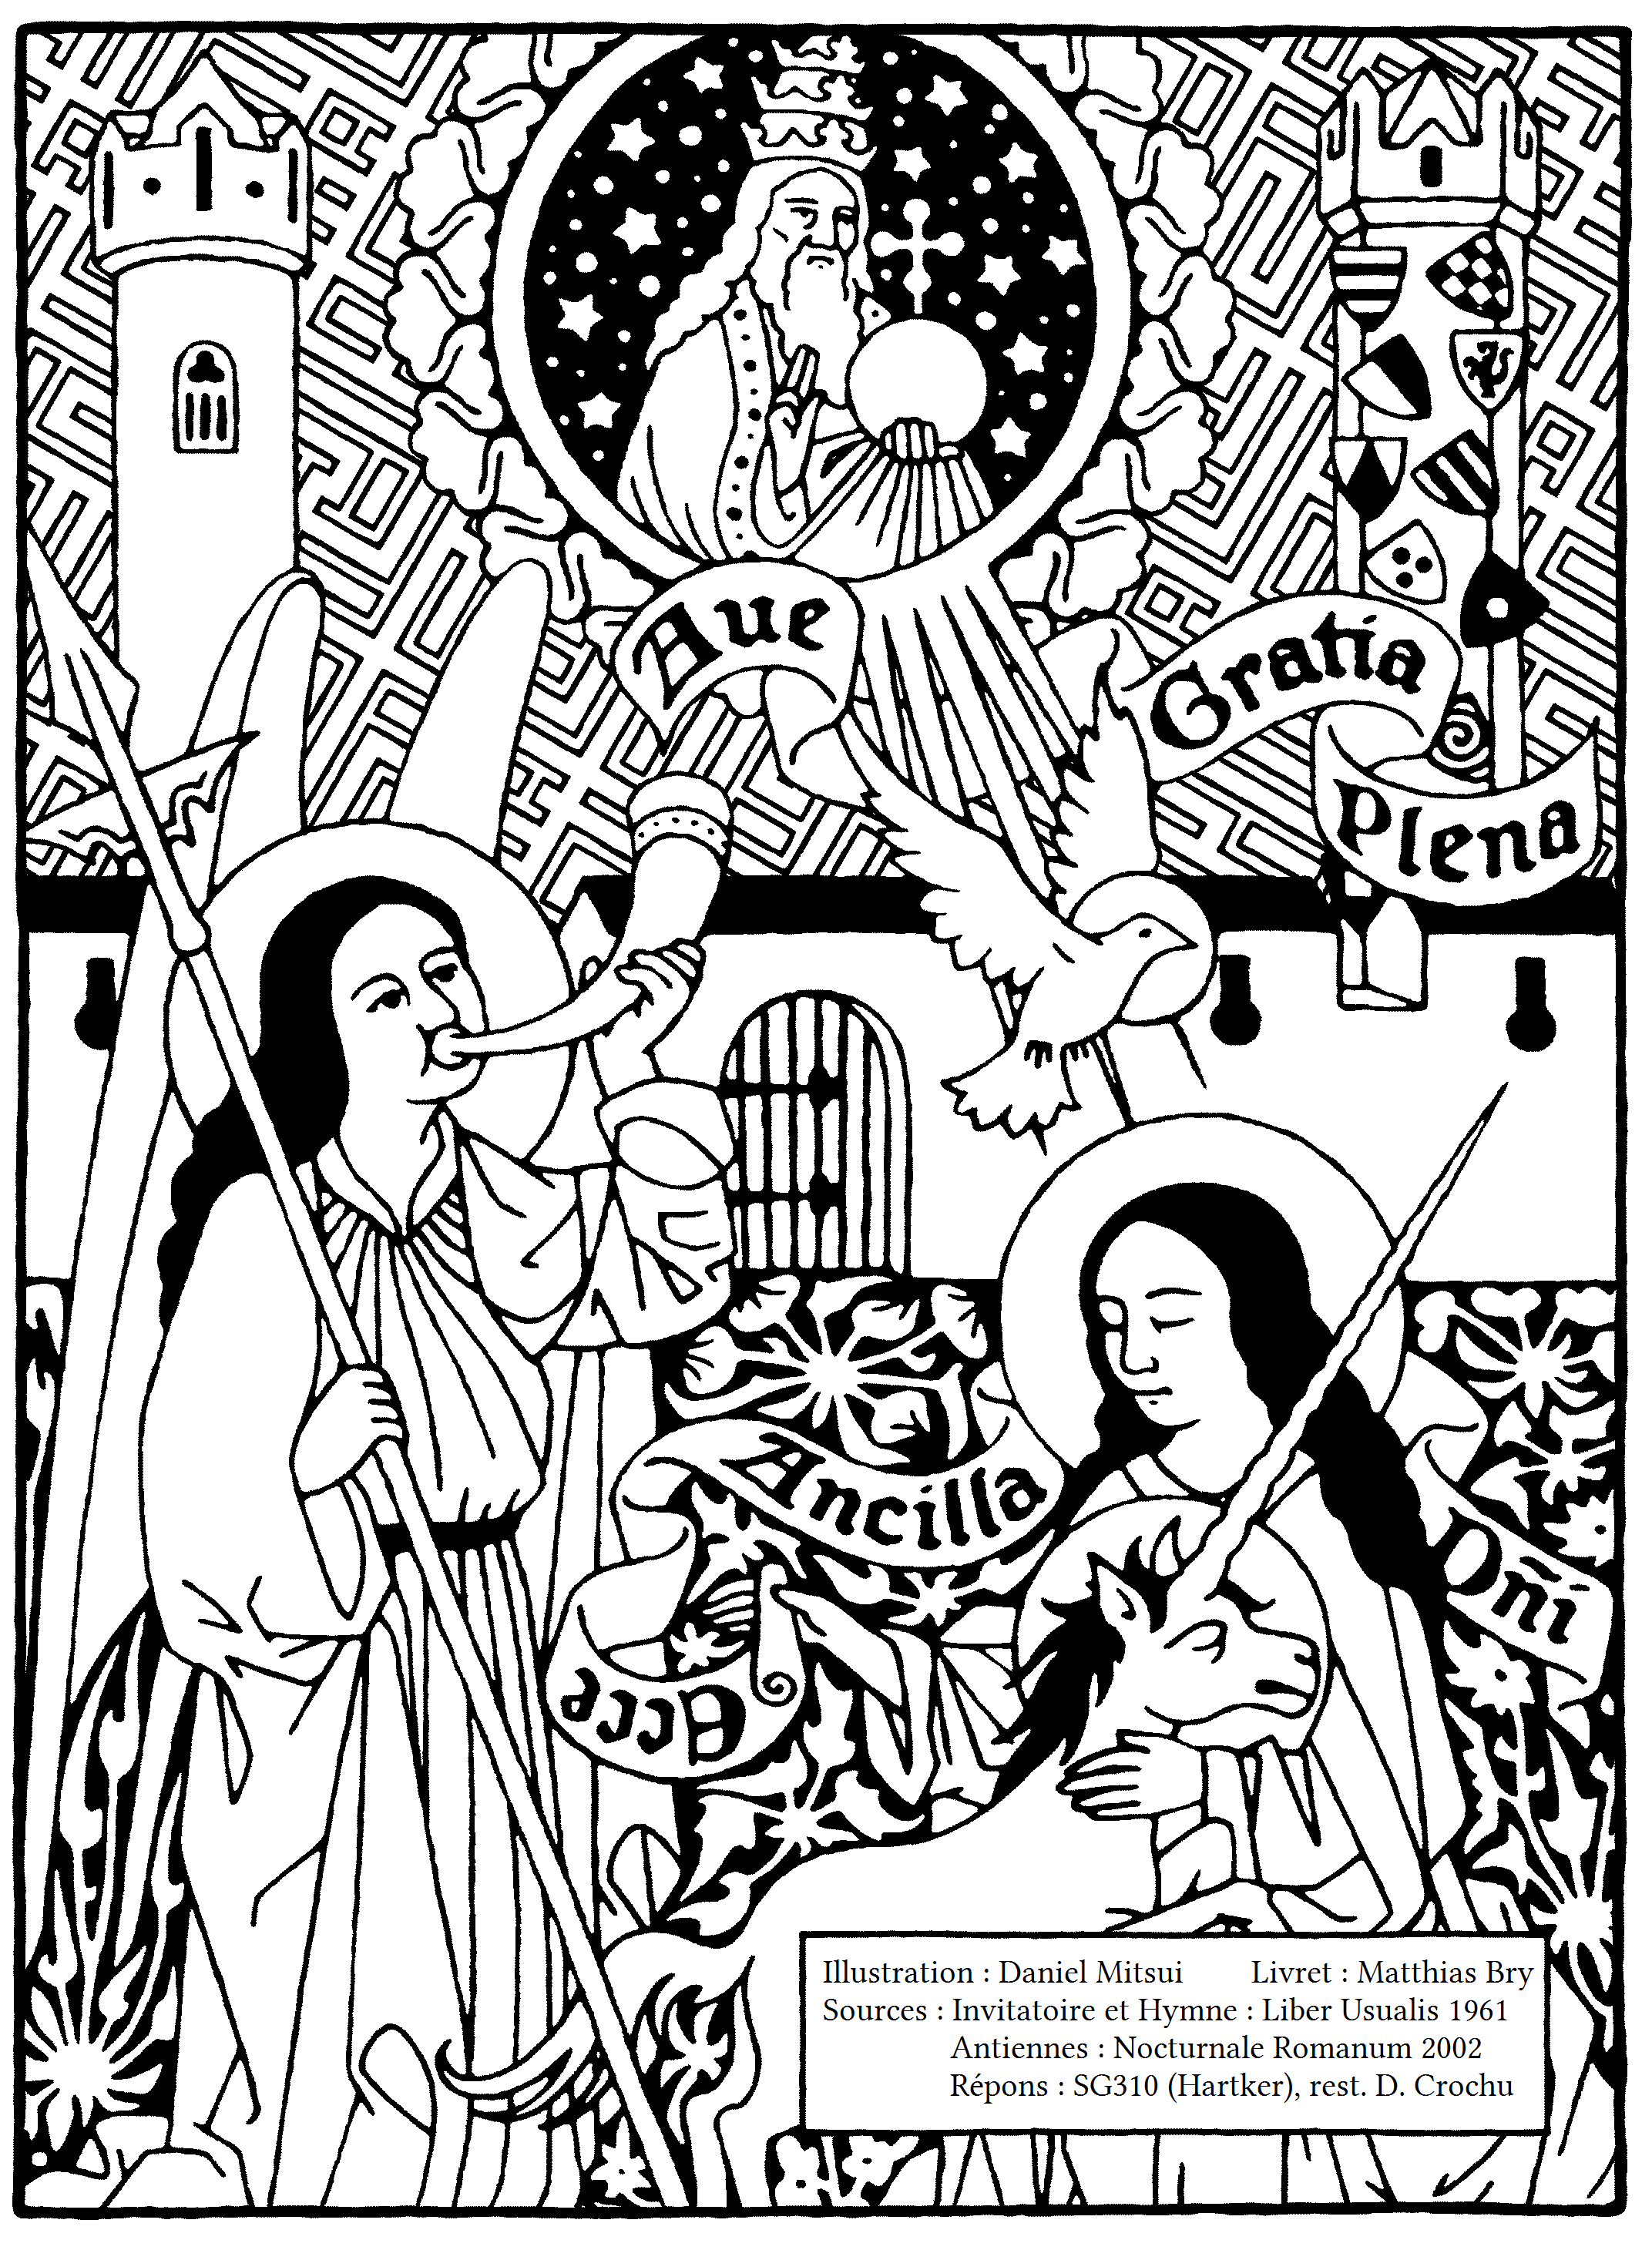
\includegraphics[width=13cm]{4ecouv.png}
\end{adjustwidth}
\end{document} 
